\scanpage{92}
% archive foliation: 91
Si $k$ n'est pas de car. $0$, on ne peut en
général aller en sens inverse, et
$R(\mathbf N,k)\xrightarrow{\Lambda}k[[t]]$ n'est \deleted{en général} pas injectif,
[$k$ corps de car. $>0$]

\figure{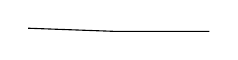
\begin{tikzpicture}\draw (0,0)--(1.1,-.04)--(2.3,-.04);\end{tikzpicture}}

On voit \deleted{que} par la formule de
Lefschetz-Weil-Grothendieck que la connaissance
de la fonction $L$ de $\unsure{(X,F)|X}$ algébrique
sur $\mathbf F_p$, \inserted{à coeff dans $F$,} \uline{équivaut} à celle de l'élément
\[
\uline{\chi}(F)=\sum(-1)^i\,\mathrm{cl}\,H^i_!(\bar X,\bar F)
\quad\text{de }R(\mathbf N,\mathbf Q_\ell)
\]
[car essentiellement cette fonction $L$ est l'image
de $\uline{\chi}(F)$ dans $1+\mathbf Q_\ell[[t]]^+$]. Lorsque
on admet les conjectures de Weil, et $F$
\inserted{est un motif,}
$\uline{\chi}(F)$ se décompose suivant les poids en
\[
\sum(-1)^i\,\deleted{\unsure{\mathrm{cl}}}\uline{h}^i_!(F),
\qquad\uline{h}^i(F)\in R(\mathbf N,\mathbf Q_\ell),
\]
et la \deleted{\unsure{connaiss.}} connaissance de $L(X,F)(t)$
\uline{équivaut} à celle des $\uline{h}^i(F)$ : les $\uline{h}^i(F)$
correspondent à la décomposition de $L(X,F)$
